\section{Motivation}
\begin{figure}
	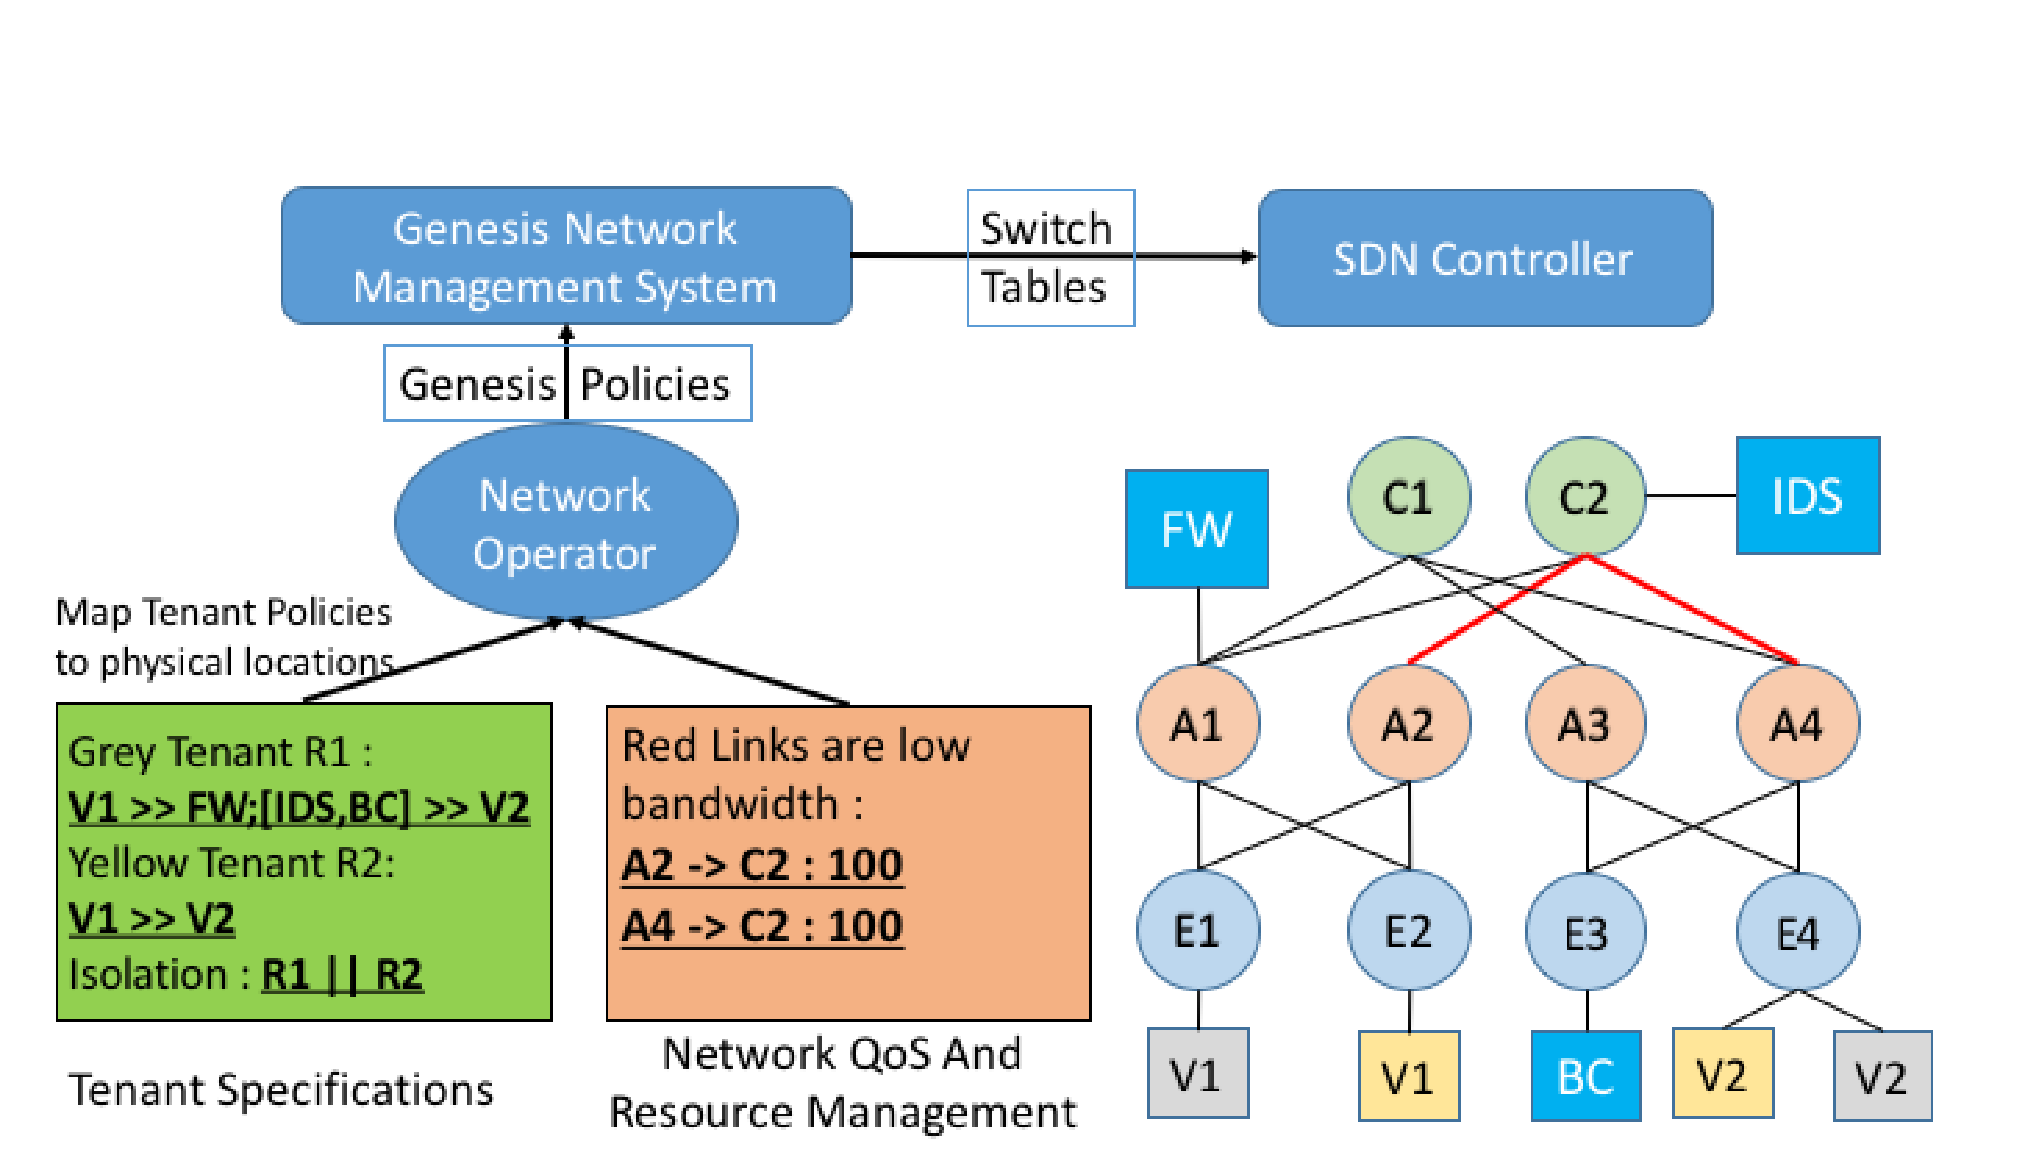
\includegraphics[width=\columnwidth,center]{figures/architecture.eps}
	\compactcaption{\Name in a multi-tenant datacenter setting.}
	\label{fig:architecture}
\end{figure}
In this section, we describe the type of policies currently supported by
Genesis. %% For simplicity, we assume a
%% multi-tenant cloud set up, where both the tenants and the provider
%% wish to realize policies over their respective networks. However,
%% these policies, and our framework, are applicable to other settings,
%% e.g., enterprise networks with different departments imposing
%% different sets of policies.
We use \Cref{fig:architecture} as a running example. This figure shows several
tenants who differ in the nature of policies they wish to realize. 
Notice that these policies reflect and, in some cases, extend the
policies that today's enterprises realize in their on-site networks, as
well as the policies that data center operators support for the different hosted
workloads~\cite{mpa-imc15}.  The policies include:

%\aditya{explain the figure here}.
%\kausik{Will do this now}

%\aditya{define flow, flow group, policy etc here}
% \aditya{need to start by saying we focus on multi-tenant clouds, although our system can apply elsewhere too}

% Operators of enterprise and multi-tenant clouds deal with policy
% requirements of different organisations and tenants, as well as
% require support to manage the network for providing QoS guarantees and
% network resource management internally, invisible to the
% tenants. Network operators need to be able to express complex policies
% in an intuitive declarative fashion, and the network management system
% must derive the individual switch forwarding behavior without
% involving the operator.


\begin{compactitemize}
\item \textbf{Reachability}. This enables network communication
  between specific groups of a tenant's virtual cloud instances,
  applications, or hosts. For example, the yellow tenant has defined a reachability
  policy for its VMs ($V1 >> V2$, which is translated  after 
  placement as $E2 >> E4$).
\item \textbf{Middlebox traversals}. A tenant may wish that traffic
  between two of her endpoints, or from another tenant, must traverse
   specific middleboxes %(locations, or logical descriptors) 
   for
  security, access control, or performance reasons. For specific
  flows, tenants can provide
  an ordered sequence of sets of middleboxes
  %\loris{flow group is not defined, group of flows or set of flows?} 
  to traverse. The flows must traverse these sets in order,
  while in a set, all middleboxes must be traversed
  and order is irrelevant.  The
  unordered set abstraction leverages the fact that middleboxes
  without dependencies in their traffic processing behavior can be
  placed in any order relative to each other~\cite{pga}. Thus the
  middlebox traversal specification outlined here generalizes the
  notion of a service chain. For example, the grey tenant in \Cref{fig:architecture}
  defines a waypoint policy $V1 >> FW; [IDS,BC] >> V2$
   which specifies that traffic must first pass through the firewall (FW),
  and then through the IDS and the byte counter (BC) in any order. 

  %% \aditya{refer here to an example in
  %%   the figure} In several cases \loris{how true is this?} the order
  %% in which these middle-boxes is traversed is not relevant and the
  %% policy language should therefore support unordered waypoints.

\item \textbf{Isolation}. Tenants may require various QoS guarantees
  that enforce varying degrees of isolation for their traffic. In the
  extreme, a tenant could require that her flow groups are not affected
  by any other tenant by strictly isolating the path of the tenant's
  flows from others' flows. In \Cref{fig:architecture}, we have two tenants
  each with one traffic class which will be isolated from one another, i.e.,
  they will not share any links in the topology. 
  A tenant could also specify isolation for a subset of her
  (performance-sensitive) flows from other flows of her own deployment
  or those belonging to other tenants; the rest of the tenants' flows
  may require no guarantees.

%%   There has been a rising emergence of 
%% multi-tenant clouds, which is more economical for tenants to use
%% rather than managing their own private datacenters. However,
%% the current Service Level Agreements (SLAs)
%% provided to tenants are centered around compute, storage, or
%% external traffic bandwidth. Lack of guarantees on the network
%% between tenant instances leads to unpredictability of performance
%% for distributed applications. Also, multi-tenant clouds are
%% susceptible to attacks on the network by malicious tenants who could
%% hog the internal network bandwidth, or conduct side-channel
%% attacks~\cite{heyyou-ccs}.
% Conventionally,
% this problem is mitigated by static rate-limiting, but it can lead
% to under-utilisation of resources.
%% Cloud provider can offer (paying) tenants various QoS guarantees
%% that enforce varying degrees of tenant isolation. In the extreme,
%% this could ensure that a tenant's performance is not affected by
%% any other tenant by strictly isolating the path of tenant's flows
%% from others' flows. \aditya{refer here to an example in
%% 	the figure} The tenant could also specify isolation for certain
%%  performance-sensitive flows, while the rest of the tenant-flows
%%   would be without guarantees with varying degrees of pricing. 
%%   Thus, support for isolation is an important feature in multi-tenant 
%%   networks. 
 
%TODO : MODIFY Synthesis of waypoints to support logical waypoints
%% Since, cloud tenants do not have a view of the actual physical
%% topology, the policy requirements for tenants are at a coarser level
%% of control. While support for the above policies can be used to satisfy tenant
%% SLAs, network operators can benefit from a fine-grained
%% control of network resources, integrated with support for tenant specifications 
%% for effective management of the network. \newline

%\loris{is there a reason why this is not in the itemize?} 
%\kausik{This is not a tenant policy, but an operator feature, so separate from itemize.}
\item \textbf{Network Resource Management}. While support for the above
policies can be used to satisfy tenant SLAs, network operators can
benefit from a fine-grained control of network resources. Support for
resource management integrated with tenant specifications is useful.
For instance, to aid traffic engineering, the network
operator may specify policies constraining the maximum number of
tenant flows that can traverse a given link or sets of links in the
network. She may also wish to ensure that traffic from some sensitive
applications does not contend for bandwidth on constrained links with
elastic traffic from batch applications. For example, in \Cref{fig:architecture},
there are two low-bandwidth links in the datacenter, and the operator
specifies policies to ensure that flows traversing $A2 \rightarrow C2$ 
and $A2 \rightarrow C4$ do not exceed the link capacity of 100.
          %% capacity
          %% of certain links such that tenant flows using the link do
          %% not exceed the capacity of the link. Such policies can be
          %% useful to ensure the low bandwidth links are not used by
          %% more tenants such that their performance is affected and
          %% can be used to provide bandwidth guarantees to tenants.
  Likewise, to tackle hardware heterogeneity operators can specify
  switch constraint policies, like the size of the rule table, to
  restrict the number of flows traversing a particular switch or set
  of switches.
\end{compactitemize}
%\item \textbf{Network Maintenance}: \aditya{this whole para does not
%    parse and needs updating} Operators on a regular basis perform link and
%  switch maintenances, and need to ensure that during maintenance, the network still
%  conforms to the SLAs of the tenants and resource capacity
%  policies.   \aditya{the following sentence does not make sense} Using Genesis, the operator
%  can specify the links and switches that will be down for maintenance, and Genesis can synthesize 
%  the rules for the updated network with all policies satisfies, which then can be pushed to 
%  the network before maintenance. 
%\end{itemize}

The above set of policies may evolve over time as operators attempt to
meet new objectives, or tenants impose new kinds of
requirements. Today, realizing these policies requires painstaking,
often manual configuration in network devices. This is incredibly
tedious---the configuration files can run into 1000s of lines, and
intricate dependencies may have to be configured across
devices~\cite{benson:complexity:nsdi2009,mpa-imc15}. This process is also highly 
error prone.

Providing support for realizing these policies using existing SDN
programming languages like Pyretic and Frenetic is challenging,
because these policies are global and cannot be enforced by
programming individual behaviour of switches. Existing SDN-based
network management systems~\cite{simple,merlin,oneswitch} are tailored
to support specific policies such as middlebox placement, bandwidth
and resource constraints. As such they lack generality and
extensibility.

Our goal is to design a system that allows these, and a variety of
hitherto unseen, policies to be specified in a simple, declarative
manner, and abstracts away data plane enforcement and the intricacies
thereof.
  
\subsection{Synthesis} \label{sec:synthesis} 

\begin{table}[!t]
\begin{small}
	\begin{center}
		\begin{tabular}{m{7.8em}  m{15.9em} } 
			{\bf Policy} & {\bf Description} \\ 
			\hline
			Reachability & There is a path from router $src$ to router $dst$ for destination $\lambda$ \\ \hline
			Reachability with \newline Ordered Waypoints & The path  from $src$ to $dst$ for destination $\lambda$ 
			traverses some switch in the set $W_1$, \ldots, then some switch in the set $W_k$.\\ \hline
			Traffic Isolation & Paths of two reachability policies $R1$ and $R2$ do not share  links \\ \hline
			Traffic Engineering  & Minimize total/max link utilization \\
		\end{tabular}
	\end{center}
	\compactcaption{\genesis path-based policy support.} \label{tab:policysupport} 
\end{small}
\end{table}


%\section{Policy Support} \label{sec:policy}
%We design a language GPL (Genesis Policy Language) for network operators to express the desired end-to-end policies in a declarative manner which is interpreted by the Genesis synthesizer to find the forwarding rules for the network topology which enforce the input policies (\cref{fig:arch}). Genesis supports the following policies : 
%% Figure of GPL's syntax
%\begin{enumerate} 
%	\item \textbf{Reachability}: $predicate : src >> dst$ \\
%	This policy specifies the packets satisying $predicate$ have ingress router $src$ and egress router $dst$, and requires rules forwarding packets satisfying $predicate$ from $src$ to $dst$. There must be no forwarding loops in the network. 
%	\item \textbf{Waypoint}: $predicate : src >> W >> dst$ \\
%	The waypoint policy is a stronger reachability policy, and specifies that packet satisfying $predicate$ with ingress router $src$ and egress router $dst$ must pass through the set of waypoints $W$ in no particular order. The waypoint policy helps operators and tenants to specify the middleboxes the packets must traverse through without worrying about order, or having to use header tags to enforce a particular order \cite{flowtags}. 
%	\item \textbf{Traffic Isolation}:  $R1 \ || \ R2$ \\
%	The traffic isolation policy ensures that the . This policy can be used to provide fairness guarantees, since the paths of $R1$ and $R2$ don't share a link, the bandwidth used by $R1$ will not affect the bandwidth used by $R2$ and vice-versa. The condition of sharing a link in the same direction is due to the fact that links are full-duplex so, traffic flowing in one direction is not affected by the traffic flowing in the other direction.
%	\item \textbf{Security Isolation}: $R1 <> R2$ \\
%	The security isolation policy is stronger than the traffic isolation policy, and ensures that the path of the reachabiltiy/waypoint policies $R1$ and $R2$ do not share a link in both directions for increased security.
%	\item \textbf{}: $sw_1 \rightarrow sw_2 : capacity$ \\
%	The link capacity policy specifies that the capacity for link $sw_1 \rightarrow sw_2$ is $capacity$, and the weights of flows traversing the link in the direction of $sw_2$ do not exceed the capacity of the link.  
%	\item \textbf{Switch Table Size}: $sw : size$ \\
%	The router table size policy is used to specify the size of the forwarding table of the router $sw$ and ensures that the number of flows traversing through $sw$ does not exceed $size$ as each flow would require a forwarding rule at the switch.
%\end{enumerate}


We design \name, a general network management system that 
by performs {\em synthesis} of switch forwarding
rules to enforce the above set of end-to-end policies . The architecture of \name
is shown in \Cref{fig:architecture} and the 
language GPL used to specify policies
is shown in \Cref{tab:policysupport}.

Unlike previous efforts in the synthesis space (see~\cite{netgen,merlin}), \Name is
not tailored to specific formalisms such as regular expressions and
this aspect makes it {\em modular} and {\em easy to extend}.
%and allows to devise specific
%techniques for each type of policies. 
To draw an analogy with SMT solvers, \Name can be seen as a constraint
solver that allows the addition of different types of policies
(respectively, the theories in SMT) and that allows the design of
optimizations based on the properties desired by 
  operators using \Name. 
  
  Our work is motivated by recent advances in program synthesis, i.e.,
  the task of discovering an executable program from user intent
  expressed in the form of some constraints. There are three key
  dimensions to synthesis: the kind of constraints that it accepts as
  expression of user intent, the space of programs over which it
  searches, and the search technique it employs. Program synthesis has
  seen limited applications to networks~\cite{netegg,decentralize},
  specifically to controller synthesis. These systems synthesize the
  behavior of individual switches (e.g., learning switches or
  firewalls); furthermore, these techniques apply to networks
  operating in a reactive mode (where the first packet of a connection
  is processed by the controller to determine the actions to
  employ). Such switch-centric approaches are too constraining and
  cannot be applied to realize network-wide objectives.

\Name\ leverages synthesis at a high level: given a set of
policies which describe user intent, the search space is the space of
all forwarding plane configurations and the search technique involved
is SAT/SMT solving. The solution is translated to switch rules installed via a skeleton controller.

This approach is appealing for the following reasons: 

(1)
Policies useful to operators are \emph{proactive} (i.e., they are not
dependent on the actual packet flow), and our synthesis approach
naturally aligns with such proactive policies.

%  and this enables enforcing policies by synthesis
% of switch-table rules, and using a skeleton SDN controller to deploy
% the forwarding rules to the switches. In contrast, in trying to
% synthesize reactive policies (like a firewall), the controller needs
% to store the state of flows it has received and have a control module
% following the specifications \aditya{huh? this doesn't make sense...},
% which is an interesting synthesis problem, but orthogonal to our
% approach.

(2) Correct policy enforcement is challenging due to different
objectives for each of the policies - ensuring isolation between flows
may lead to overshooting capacity and vice-versa - and is a common
cause of incorrect configurations in networks.  Our approach removes
the need for a verification step in which the operator has to
``check'' whether an attempted configuration meets the desired
policies.  By using a formal reasoning technique, we are able to
consider the space of all forwarding configurations and find a
solution which is \emph{correct by construction}, i.e., it adheres to
satisfying a diverse set of policies, eliminating the room for error
by the network operator.

(3) Automatically enforcing policies is a task with
\emph{high theoretical complexity}. 
For example, enforcing isolation policies
is as hard as solving
graph-coloring, a well-known
NP-complete problem (proof has been omitted for brevity).
%, which means
%that any system solving this would need to exhaustively search the
%space of all forwarding plane configurations. 
Many search techniques can be used to find the forwarding rules when
handling a particular class of policies, but when multiple types of
policies are combined (isolation, middlebox traversal, capacity
constraints), devising good search techniques becomes challenging.
Thanks to the many engineering efforts, SMT solvers abstract away most
of this complexity and allow us to unify the search objectives for
every policy into a generalized search technique.
%Thus, by reducing this problem to a SMT instance and
%leveraging fast off-the-shelf SMT solvers developed over years of
%research, \Name can provide support for diverse policies required by
%network operators. 
Crucially, \Name can be extended with ease to
support new policies without requiring changes to the underlying search
techniques.
%% \loris{I would like to convey that we are in some sense a Network solver module policy,
%% in the sense that we support theories (the policies) and now people can work on engineering
%% the solver for different classes of policies.
%% }
%% \kausik{To flow from this subsec to the next? Support for policies is 
%% 	inbuilt, but operators can engineer tactics to suit their needs. Is this what you want to convey?}
%% \loris{I found many words used to address the same concept:
%% enforce the policies, synthesize rules, etc...
%% try to be uniform or it's quite hard to understand what is being done.
%% } 
%% \kausik{I think "enforce policies" would be better? The title explains the rest.}

\subsection{Performance Challenges} \label{sec:performance}

One of the key challenges of \Name is the synthesis
performance. 
Due to the rich set of policies supported by \Name,
finding a consistent set of switch forwarding rules 
has, in the worst case, exponential time complexity in
the number of policies.
Moreover, since policies such as isolation affect
the paths of many different flows, it is not possible to incrementally synthesize
the forwarding rules corresponding to each flow. NetGen~\cite{netgen}
synthesizes incremental changes to forwarding tables for individual
flows, however 
it does not support isolation.
Despite the recent advances in SMT solvers, to make
the synthesis problem feasible in practice
there is a need to improve the performance of the solver
using techniques that are specific to policy enforcement in networks.
We propose various techniques leveraging
\emph{domain-specific} knowledge to improve synthesis performance. 

First, we propose the idea of \emph{tactics} (\Cref{sec:tactic}),
which are search strategies that leverage the tiered network structure
of datacenter topologies.
%, to specify properties of the paths for the reachability
%policies.  
Tactics allow network operators to specify a
high-level description on the set of paths allowed for reachability
policies.  Tactics are expressed as simplified forms of
regular expressions, which can be used to simplify the set of constraints provided to
the solver.  In particular, one can eliminate constraints that cannot
be true for any of the paths accepted by the language of the regular expression. We
find that this can result in 1.5x-400x speedup for different workloads.

Second, we propose a heuristic procedure that takes advantage of the fact that in 
datacenter topologies the large
interconnect of links can lead to multiple solutions 
to enforce the provided policies.  
We design a heuristic procedure called \emph{optimistic}
synthesis (\Cref{sec:optimistic}) which leverages the structure of
isolation policy interactions among tenants to partition the input
policies into components and synthesize these components separately and
faster than the complete problem. To improve the effectiveness of the
heuristic, whenever the SMT solver fails to find a solution we extract
the unsatisfiability core produced by the SMT solver and 
add it to our set of constraints to quickly converge to a correct solution.
Informally, the unsatisfiability core can be viewed
as a set of constraints that describes why there wasn't a feasible solution~\cite{unsatcores}.

